
% === Pali ===

\cleartoverso

\vspace*{30mm}

\begin{verse}

\verseref{1}
\emph{kathaṁdassī kathaṁsīlo\\
upasantoti vuccati}\\
\emph{taṁ me gotama pabrūhi\\
pucchito uttamaṁ naraṁ}

\verseref{2}
vītataṇho purā bhedā\\
pubbamantamanissito\\
vemajjhe nupasaṅkheyyo\\
tassa natthi purakkhataṁ

\verseref{3}
akkodhano asantāsī\\
avikatthī akukkuco\\
mantabhāṇī anuddhato\\
sa ve vācāyato muni

\verseref{4}
nirāsatti anāgate\\
atītaṁ nānusocati\\
vivekadassī phassesu\\
diṭṭhīsu ca na nīyati

\verseref{5}
patilīno akuhako\\
apihālu amaccharī\\
appagabbho ajeguccho\\
pesuṇeyye ca no yuto

\verseref{6}
sātiyesu anassāvī\\
atimāne ca no yuto\\
saṇho ca paṭibhānavā\\
na saddho na virajjati

\verseref{7}
lābhakamyā na sikkhati\\
alābhe ca na kuppati\\
aviruddho ca taṇhāya\\
rasesu nānugijjhati

\verseref{8}
upekkhako sadā sato\\
na loke maññate samaṁ\\
na visesī na nīceyyo\\
tassa no santi ussadā

\verseref{9}
yassa nissayatā natthi\\
ñatvā dhammaṁ anissito\\
bhavāya vibhavāya vā\\
taṇhā yassa na vijjati

\verseref{10}
taṁ brūmi upasantoti\\
kāmesu anapekkhinaṁ\\
ganthā tassa na vijjanti\\
atarī so visattikaṁ

\verseref{11}
na tassa puttā pasavo\\
khettaṁ vatthuñca vijjati\\
attaṁ vāpi nirattaṁ vā\\
na tasmiṁ upalabbhati

\verseref{12}
yena naṁ vajjuṁ puthujjanā\\
atho samaṇabrāhmaṇā\\
taṁ tassa apurakkhataṁ\\
tasmā vādesu nejati

\verseref{13}
vītagedho amaccharī\\
na ussesu vadate muni\\
na samesu na omesu\\
kappaṁ neti akappiyo

\verseref{14}
yassa loke sakaṁ natthi\\
asatā ca na socati\\
dhammesu ca na gacchati\\
sa ve santoti vuccatīti

\end{verse}

% === Slovenian ===

\chapter[Purābheda Sutta]{{kama-sutta-gray.png}{ucenje-2.png}}

% Učenje o pred razpadom

\begin{verse}

%\vFirst
%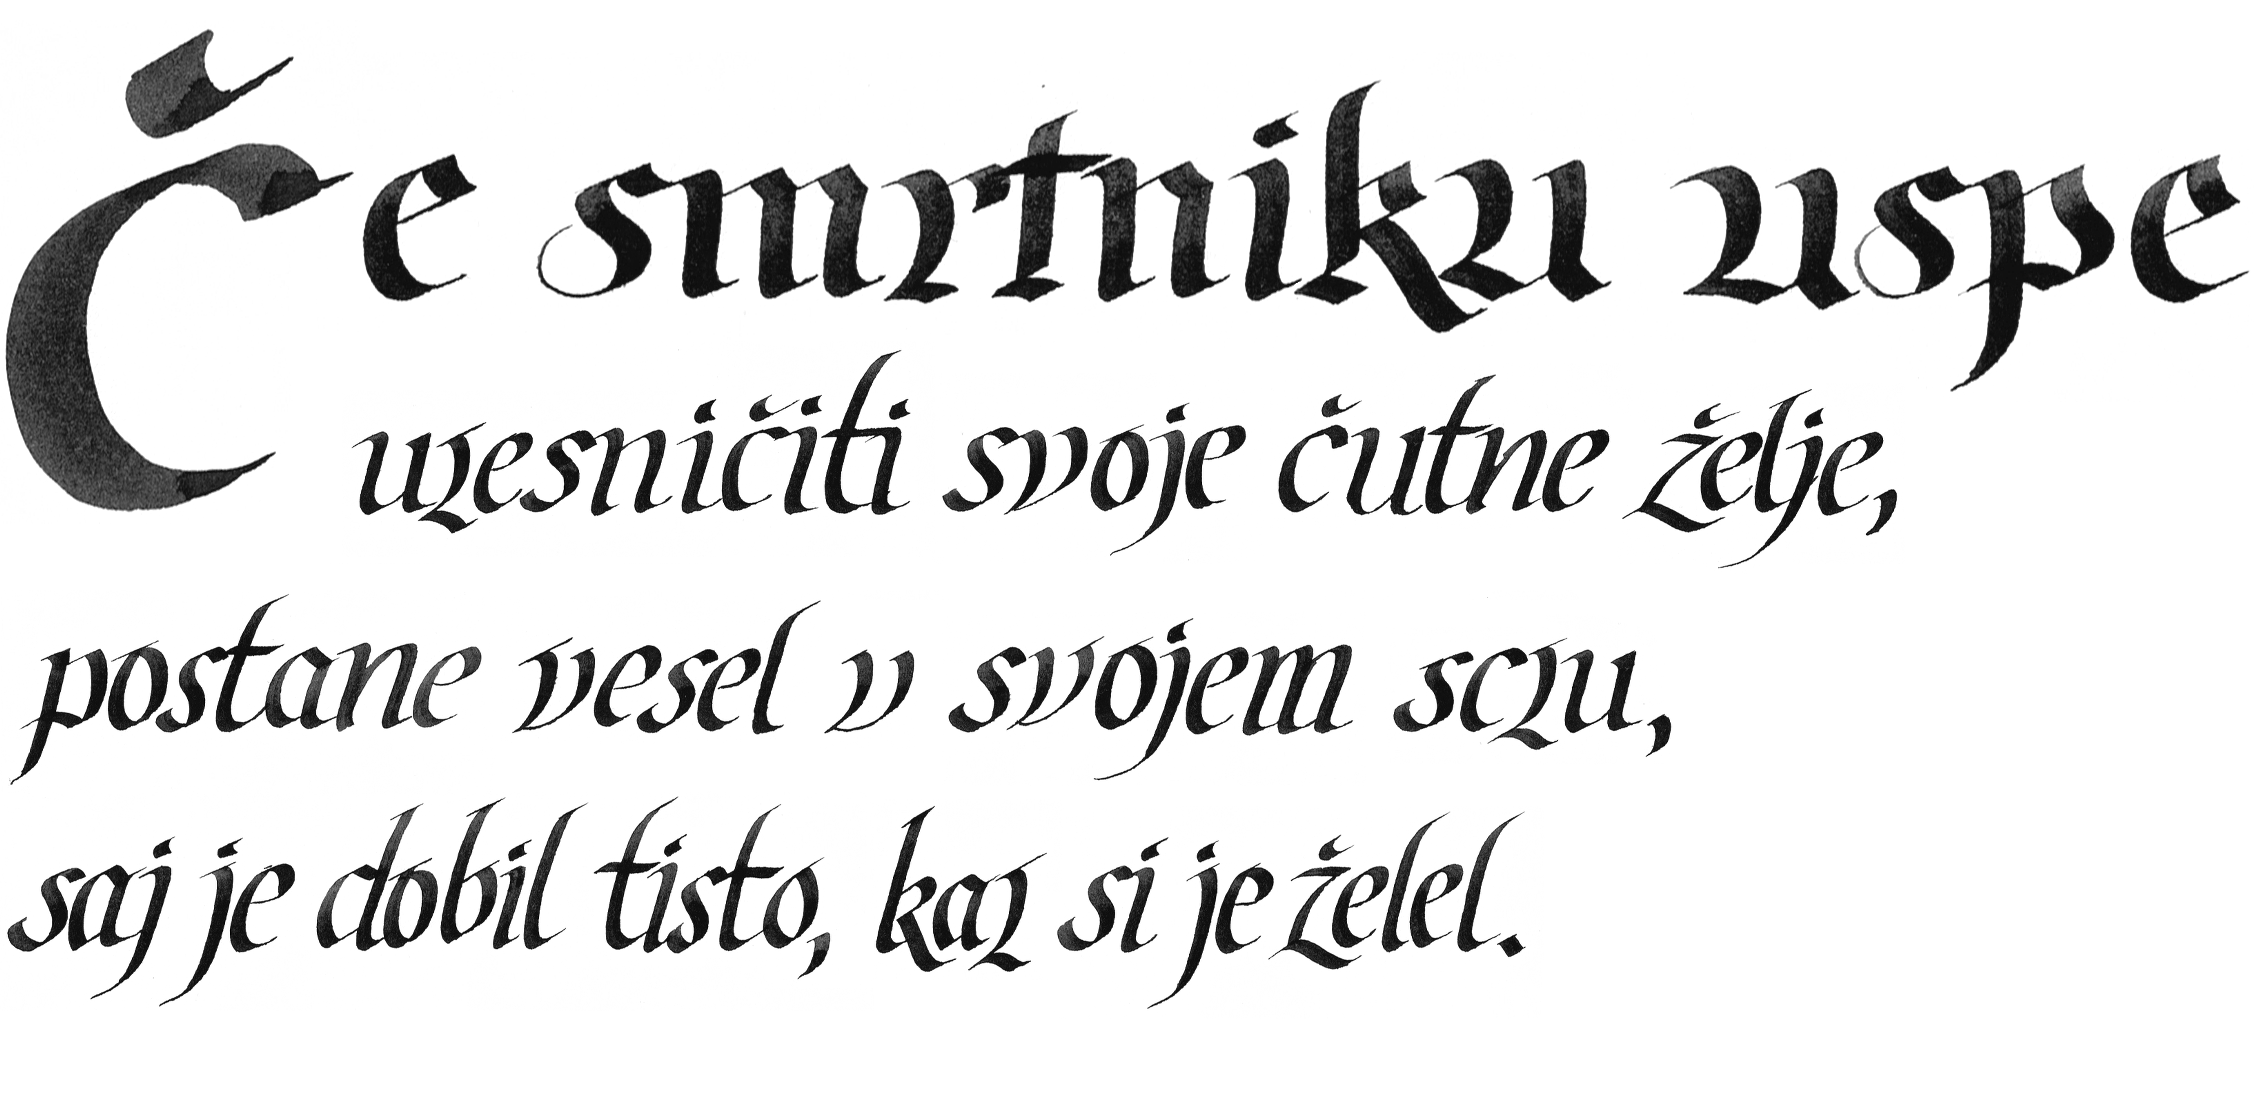
\includegraphics[scale=0.3]{ce-smrtniku-gray.png}

\verseref{1}
\emph{S kakšno vizijo, s kakšno moralo\\
se lahko komu pravi, da je v miru?\\
Povejte mi to, o Gotama.\\
Sprašujem vas o najboljšem človeku.}

\verseref{2}
S prenehanjem hrepenenja pred razpadom,\\
ni odvisen od preteklosti,\\
ni pogojen v sedanjosti,\\
si ta ničesar ne daje v ospredje.

\verseref{3}
Brez jeze in strahu,\\
brez hvale in skrbi,\\
jasen govornik ni domišljav,\\
pravi modrec, ki se obvladuje v govoru.

\verseref{4}
Brez navezanosti na prihodnost,\\
ne obžaluje preteklosti.\\
Vidi osamo med vsemi kontakti,\\
ničesar med pogledi ga ne zapelje.

\verseref{5}
Je odmaknjen, ni spletkar,\\
ni pohlepen in se ne boji izgube,\\
ni drzen, je brez odpora\\
in ni naklonjen žalitvam.

\verseref{6}
Se ne predaja prijetnostim,\\
ni naklonjen zaničevanju,\\
je blag in bistrega duha,\\
ni pobožen niti ni pasiven.

\verseref{7}
Ne vodijo ga želje po koristih\\
in ni razočaran, če le teh ni.\\
Hrepenenje ga ne ovira,\\
niti ni lakomen za okusne draži.

\verseref{8}
Za ravnodušnega in pozornega opazovalca,\\
ki se nima za enakega,\\
za boljšega ali slabšega --\\
za njega ni časti.

\verseref{9}
Za njega ni odvisnosti,\\
z razumevanjem Poti je neodvisen.\\
V njem ne obstaja hrepenenje\\
niti po obstoju niti po ne-obstoju.

\verseref{10}
Takemu pravim, da je v miru:\\
takem, ki si ne želi čutnih užitkov,\\
v katerem ni najti nobenih vezi,\\
saj je za seboj pustil vse navezanosti.

\verseref{11}
Zanj ne obstajajo sinovi ali živina,\\
niti polja ali lastnina.\\
Skratka, pri njem ni ničesar,\\
kar bi lahko pridobil ali zavrgel.

\verseref{12}
S tem, s čimer bi ga lahko nevedni ljudje kritizirali,\\
ali tudi misleci in sveti možje,\\
on ničesar ne daje v ospredje,\\
zato je tudi sredi kritike miren.

\verseref{13}
Je brez pohlepa in se ne boji izgub,\\
takšen modrijan se nima za nadrejenega,\\
niti za enakega niti za podrejenega.\\
Ni zapadel v predstave; on je brez predstav.

\verseref{14}
Tistemu, ki ničesar ne poseduje,\\
ki se ne žalosti, ker ničesar nima,\\
in ki ne sledi nobenim idejam --\\
le takemu se lahko resnično pravi, da je v miru s seboj.

\end{verse}

% === Pali ===

\clearpage
\begin{verse}

\verseref{5}

\end{verse}

% === Slovenian ===

\clearpage
\begin{verse}

\verseref{5}

\end{verse}

